\section{Phân cụm và đánh giá kết quả}
\label{sec:e}

\subsection{Thiết lập thực nghiệm}
\paragraph{Thuật toán.} \textbf{K-Means} (\var{n_init}=50, \var{random_state}=42) là thuật toán chính: khoảng cách Euclid trên ma trận đã chuẩn hóa đúng là điều bước chuẩn bị đã thực hiện, tái lập được và tâm cụm đọc được.
Thuật toán thứ hai là \textbf{phân cụm phân cấp trên khoảng cách Gower} (không cần ma trận số, dùng thang riêng) để xem kết luận có chỉ đúng với K-Means hay không. Chưa dùng DBSCAN/GMM; K-Prototypes không chạy được (thiếu thư viện \texttt{kmodes}).

\paragraph{Các nhánh so sánh.} Cả năm nhánh dùng \textbf{cùng 260 khách}; số cột khác nhau và là một phần của khác biệt cần đọc (Bảng~\ref{tab:branches}). B1 là nền công bằng: biến đổi \emph{tối thiểu} để K-Means chạy
(điền trung vị, one-hot, mã hạng, z-score mọi cột); B0 bỏ cả z-score để thấy riêng tác động của thang đo; L2 là dữ liệu sau tiền xử lý với đúng biến đổi của B1 (tách đóng góp của tiền xử lý khỏi chuẩn bị); L3 là $X_{\text{main}}$ của bước chuẩn bị.
REF là dữ liệu sạch D0 qua đúng pipeline của bước chuẩn bị: \textbf{mốc trần}, không phải một phương pháp.

\begin{table}[htbp]
\centering\small
\caption{Các nhánh so sánh (cùng 260 dòng).}
\label{tab:branches}
\begin{tabularx}{\linewidth}{llcX}
\toprule
Nhánh & Vai trò & Số cột & Dữ liệu và biến đổi\\
\midrule
B0 & Phụ & 20 & D3, điền trung vị, one-hot, mã hạng, \emph{không} chuẩn hóa\\
\textbf{B1} & \textbf{Trước xử lý} & 20 & B0 + z-score mọi cột\\
L2 & Phụ (riêng tiền xử lý) & 21 & Dữ liệu sau tiền xử lý, cùng biến đổi như B1 (\texttt{unknown} là một mức)\\
\textbf{L3} & \textbf{Sau xử lý, chuẩn bị} & 19 & $X_{\text{main}}$ (log1p, z-score, one-hot $\times\,w$, bỏ total\_spend)\\
REF & Mốc trần & 19 & D0 sạch qua đúng pipeline của bước chuẩn bị\\
\bottomrule
\end{tabularx}
\end{table}

\paragraph{Chọn $k$ và chỉ số.} $k$ được chọn \emph{chỉ bằng chỉ số nội tại} (Silhouette cao nhất, $k=2,\dots,8$); nhãn phân khúc ẩn không tham gia chọn $k$, tham số hay biến. Vì 4 là số phân khúc do ta thiết kế, kết quả được báo cáo ở cả $k$ chọn theo nội tại và $k=4$ cố định (để so cùng $k$).
Chỉ số ngoài: ARI, NMI, purity so với phân khúc ẩn. Chỉ số nội tại: Silhouette, Davies--Bouldin, Calinski--Harabasz ở thang riêng \emph{và ở thang chung} $X_{\text{main}}$; chỉ thang chung mới so sánh được giữa các nhánh.
Độ ổn định: ARI giữa cụm trên mẫu con 80\% (30 lần) và cụm đầy đủ; ARI giữa 20 lần chạy \var{n_init}=1 và lần tốt nhất. Khoảng tin cậy 95\% bằng bootstrap 1000 lần theo dòng, ghép cặp giữa các nhánh.

\subsection{Kết quả}
\paragraph{Chọn số cụm.} Trên dữ liệu thô, Silhouette ở thang riêng tăng gần liên tục theo $k$ và B1 chọn $k=7$ (Silhouette $0{,}180$, có một cụm chỉ 1 dòng); L2 cũng chọn $k=7$; B0 chọn $k=2$ với Silhouette $0{,}948$ và cụm $257/3$, một phân hoạch suy biến.
Chỉ L3 có đỉnh rõ tại đúng $k=4$ (Silhouette $0{,}299$; Davies--Bouldin thấp nhất $1{,}277$), như dữ liệu sạch (Hình~\ref{fig:e_k}).

\begin{figure}[htbp]
\centering
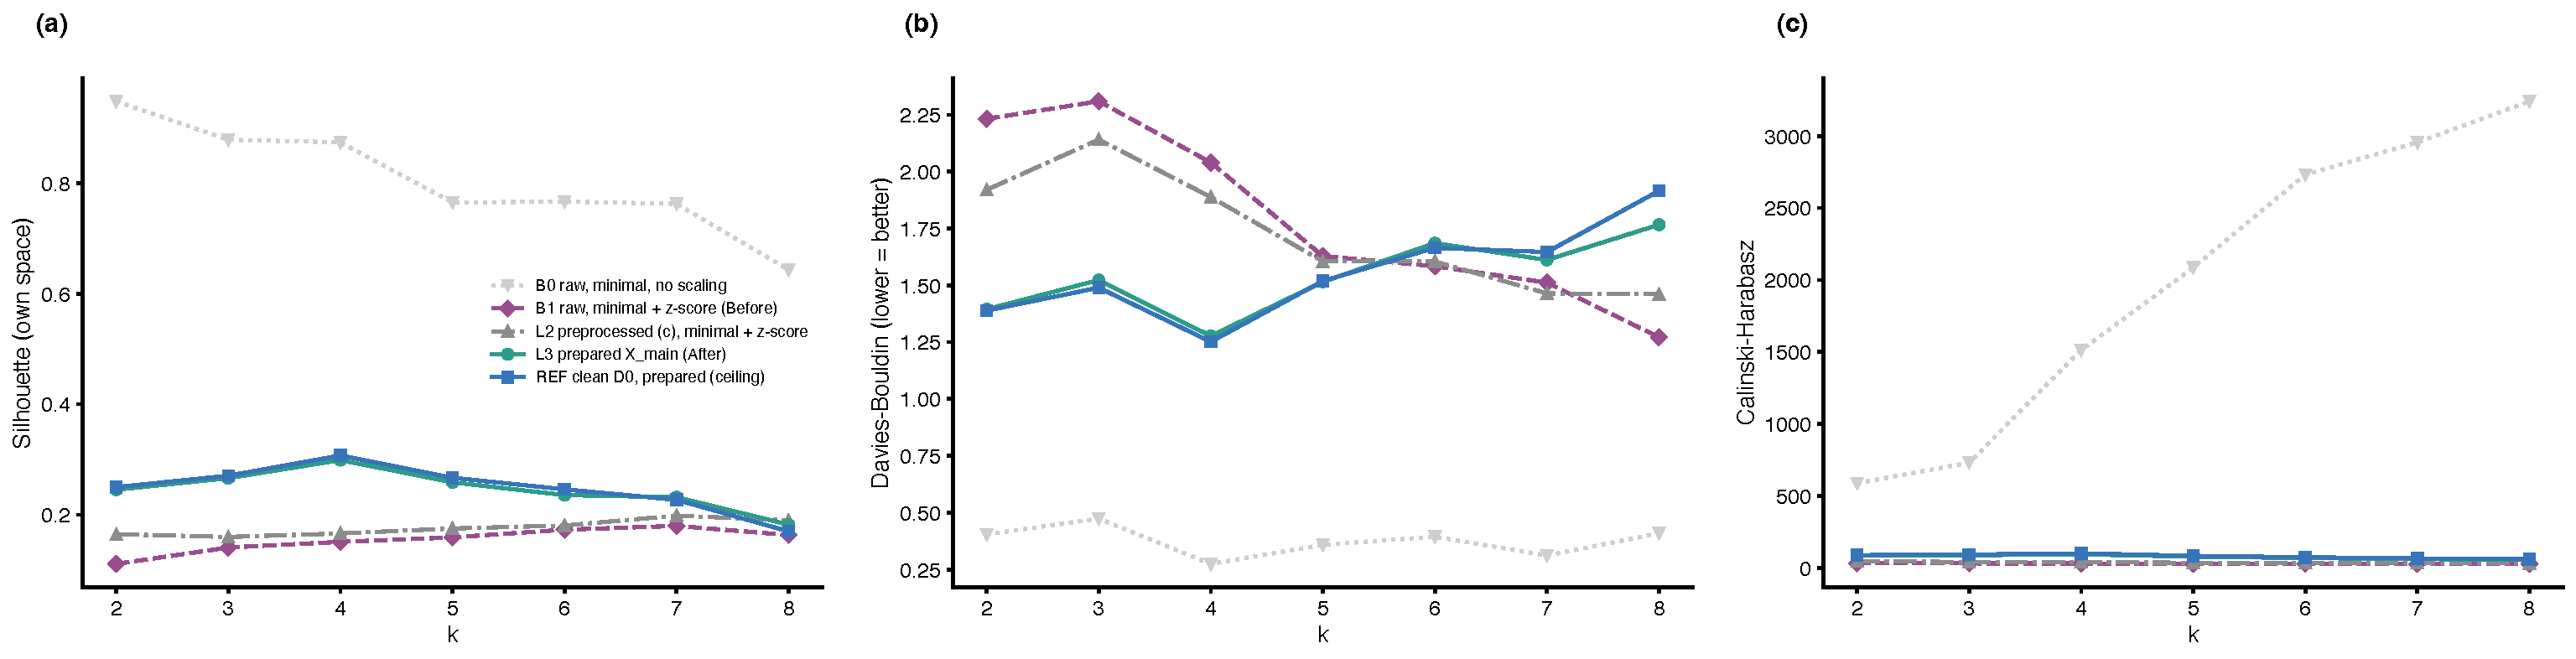
\includegraphics[width=\linewidth]{figE1_k_selection.pdf}
\caption{Chọn $k$ theo Silhouette (cao tốt), Davies--Bouldin (thấp tốt) và Calinski--Harabasz (cao tốt), ở thang riêng của từng nhánh. Giá trị Silhouette thang riêng của B0 (0,95) là của một phân hoạch suy biến.}
\label{fig:e_k}
\end{figure}

\paragraph{Chất lượng phân cụm.} Bảng~\ref{tab:e_k4} và Hình~\ref{fig:e_ext} cho kết quả ở $k=4$. B1 đạt ARI $0{,}611$; sau tiền xử lý (L2) $0{,}701$; sau chuẩn bị (L3) $0{,}745$; dữ liệu sạch (REF) $0{,}777$.
Silhouette ở thang riêng không so sánh được giữa các nhánh (B0 có $0{,}874$ nhưng ARI $0{,}035$); ở thang chung $X_{\text{main}}$ Silhouette tăng từ $0{,}254$ (B1) lên $0{,}299$ (L3) và Davies--Bouldin giảm từ $1{,}449$ xuống $1{,}277$.

\begin{table}[htbp]
\centering\small
\caption{K-Means, $k=4$. ARI có khoảng tin cậy 95\% bootstrap. Ổn định: ARI mẫu con 80\% (trung bình $\pm$ sd) và ARI giữa các lần chạy \var{n_init}=1 (trung bình / thấp nhất).}
\label{tab:e_k4}
\begin{tabular}{lcccccc}
\toprule
Nhánh & ARI [CI 95\%] & NMI & Purity & Sil. thang chung & Kích thước cụm & Ổn định\\
\midrule
B0 & 0,035 \CI{0,016}{0,061} & 0,130 & 0,358 & 0,130 & 245/12/2/1 & 0,914$\pm$0,184; 1,00/1,00\\
\textbf{B1} & \textbf{0,611} \CI{0,515}{0,708} & 0,571 & 0,835 & 0,254 & 82/68/65/45 & 0,829$\pm$0,150; 0,685/0,435\\
L2 & 0,701 \CI{0,610}{0,787} & 0,664 & 0,877 & 0,274 & 82/68/67/43 & 0,949$\pm$0,039; 0,823/0,485\\
\textbf{L3} & \textbf{0,745} \CI{0,658}{0,833} & 0,698 & 0,896 & 0,299 & 77/74/63/46 & 0,970$\pm$0,017; 0,958/0,721\\
REF & 0,777 \CI{0,693}{0,856} & 0,737 & 0,912 & 0,295 & 75/74/66/45 & 0,987$\pm$0,013; 0,996/0,980\\
\bottomrule
\end{tabular}
\end{table}

\begin{figure}[htbp]
\centering
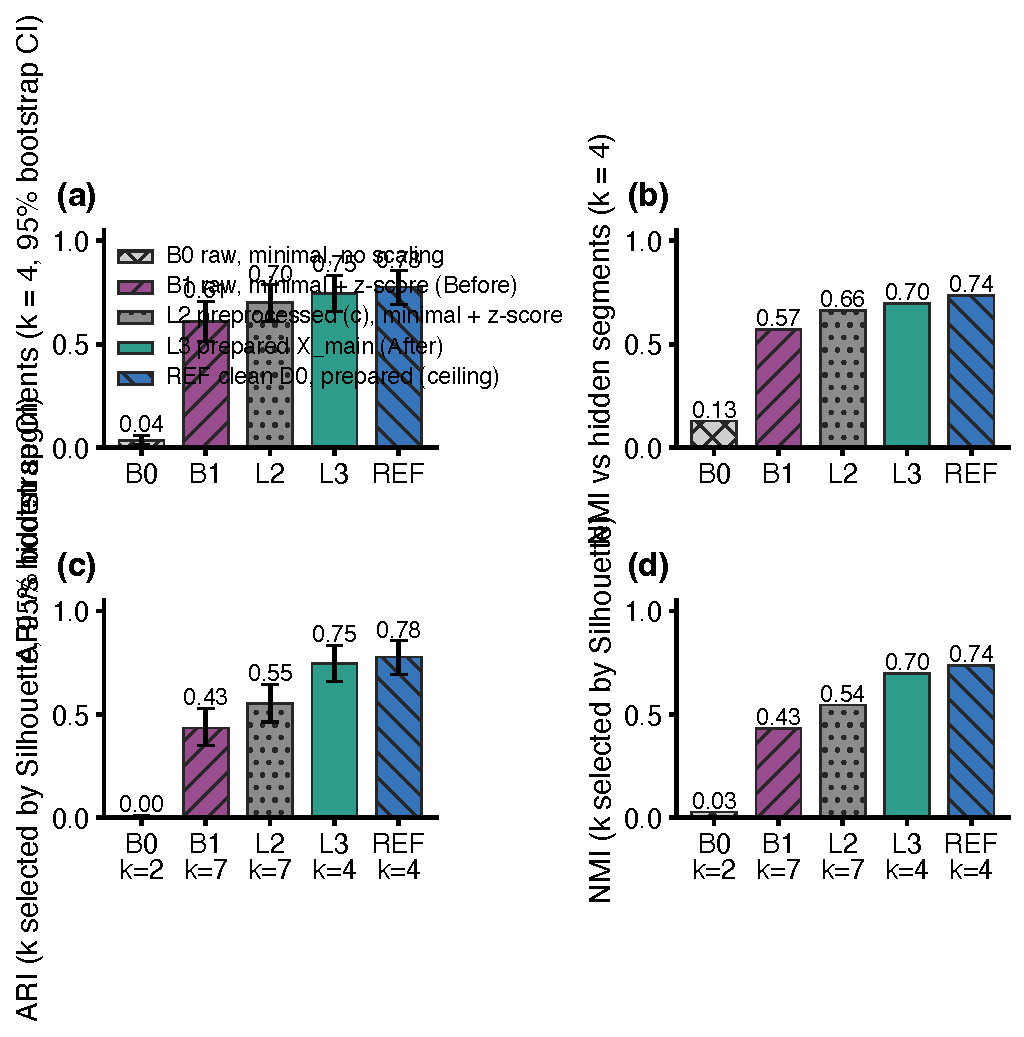
\includegraphics[width=0.9\linewidth]{figE2_external_metrics.pdf}
\caption{Chỉ số ngoài so với phân khúc ẩn. (a, b) ARI (có CI 95\%) và NMI ở $k=4$; (c, d) ARI và NMI khi $k$ chọn theo Silhouette (nhãn trục ghi $k$ được chọn).}
\label{fig:e_ext}
\end{figure}

\paragraph{Chênh lệch có ý nghĩa không?} Bảng~\ref{tab:e_diff} dùng bootstrap ghép cặp. Tổng hiệu quả tiền xử lý + chuẩn bị là rõ ràng ở cả hai thiết lập; riêng tiền xử lý có ý nghĩa; riêng chuẩn bị \emph{không} phân biệt được với 0 ở $k=4$,
và khoảng cách tới dữ liệu sạch cũng không phân biệt được với 0 ở $n=260$.

\begin{table}[htbp]
\centering\small
\caption{Chênh lệch ARI (bootstrap ghép cặp, CI 95\%).}
\label{tab:e_diff}
\begin{tabular}{lcc}
\toprule
So sánh & $k=4$ & $k$ chọn theo Silhouette\\
\midrule
L3 $-$ B1 (tiền xử lý + chuẩn bị) & $+0{,}134$ \CI{0,058}{0,206} & $+0{,}311$ \CI{0,224}{0,393}\\
L2 $-$ B1 (riêng tiền xử lý) & $+0{,}090$ \CI{0,040}{0,143} & $+0{,}117$ \CI{0,057}{0,177}\\
L3 $-$ L2 (riêng chuẩn bị) & $+0{,}044$ \CI{-0,024}{0,115} & $+0{,}194$ \CI{0,101}{0,281}\\
REF $-$ L3 (khoảng cách tới trần) & $+0{,}032$ \CI{-0,007}{0,071} & $+0{,}032$ \CI{-0,007}{0,071}\\
\bottomrule
\end{tabular}
\end{table}

Lợi ích của bước chuẩn bị nằm ở \emph{độ vững} chứ không phải ARI tại $k=4$: L3 chọn đúng $k=4$ trong khi L2 chọn $k=7$ (chênh ARI $+0{,}194$ khi $k$ chọn theo nội tại), và K-Means ít mắc tối ưu cục bộ hơn
(ARI giữa các lần chạy \var{n_init}=1: $0{,}823\to0{,}958$; thấp nhất $0{,}485\to0{,}721$).

\paragraph{Khách ``cầu nối'' quyết định trần.} Trên 213 khách thường, ARI là $0{,}812$ (B1), $0{,}869$ (L2), $\mathbf{0{,}966}$ (L3) và $1{,}000$ (REF); trên 47 khách cầu nối mọi nhánh chỉ đạt $0{,}06$--$0{,}19$ (kể cả REF $0{,}19$).
Phần cải thiện nằm ở khách thường; không phương pháp nào phục hồi được nhóm khách vốn do thiết kế nằm giữa hai phân khúc.

\paragraph{Tác động của dòng hỏng.} Ở $k=4$ trên B1, 7 dòng có ô hỏng không lập thành cụm riêng (cụm nhỏ nhất 45 dòng). Khi $k=7$ (do Silhouette chọn), xuất hiện một cụm chỉ gồm 1 dòng và dòng đó là dòng có ô hỏng. Tác hại chính của ô hỏng là gián tiếp:
làm méo thang đo và làm Silhouette chọn sai $k$.

\subsection{Đặc điểm các cụm}
Ở $k=4$, bốn cụm của L3 tương ứng bốn kiểu khách và khớp tốt với phân khúc ẩn (233/260 khách đúng cụm, 89,6\%; B1: 217/260, 83,5\%).

\begin{table}[htbp]
\centering\small
\caption{Hồ sơ cụm của L3 ($k=4$; trung vị theo đơn vị gốc của dữ liệu đã xử lý) và phân khúc ẩn chiếm đa số.}
\label{tab:e_prof}
\begin{tabularx}{\linewidth}{lrX l}
\toprule
Cụm & $n$ & Đặc điểm (trung vị) & Phân khúc ẩn\\
\midrule
1. Giá trị cao & 46 & 31,5 đơn; tổng chi 3\,093 USD; AOV 110; recency 7 ngày; discount 0,08; hạng gold; mobile; 72\% cài app & HighValue 42/46\\
2. Ít mua & 63 & 2 đơn; tổng chi 114 USD; recency 130 ngày; 2 phiên/tháng; desktop; 43\% cài app & Infrequent 54/63\\
3. Chủ yếu duyệt & 74 & 1 đơn; 17,5 phiên/tháng; 20,7 trang/phiên; bỏ giỏ 0,89; mobile; electronics; 84\% cài app & Browser 66/74\\
4. Săn khuyến mãi & 77 & discount 0,92; 17 đơn; AOV 28; tổng chi 450 USD; fashion; mobile & PromoHunter 71/77\\
\bottomrule
\end{tabularx}
\end{table}

Gợi ý nghiệp vụ suy từ hồ sơ: cụm 1 chăm sóc khách VIP; cụm 2 kích hoạt lại khách đã lâu không mua; cụm 3 tăng chuyển đổi (nhắc giỏ hàng, rút ngắn đường mua); cụm 4 khuyến mãi có kiểm soát biên lợi nhuận.
Với B1, bốn cụm tương tự nhưng lẫn nhiều hơn: 10 khách Infrequent rơi vào cụm khuyến mãi và 6 khách HighValue rơi vào cụm ít mua.

\begin{figure}[htbp]
\centering
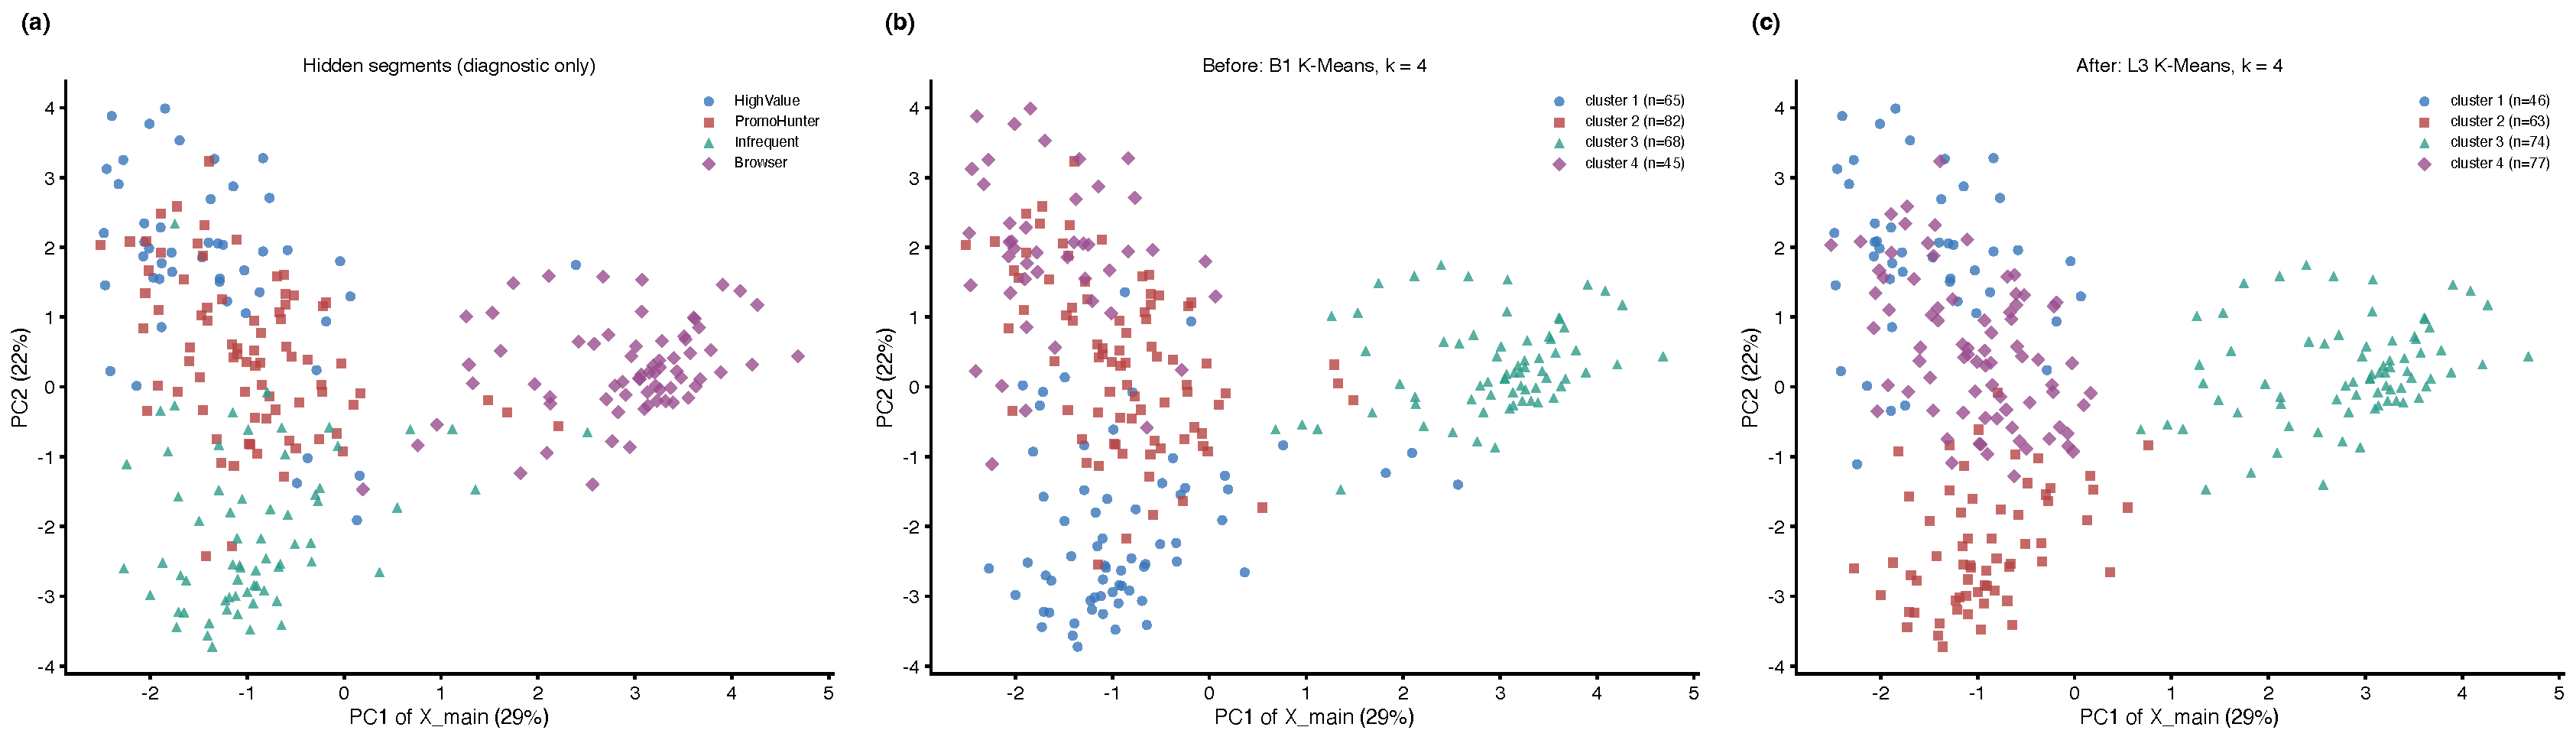
\includegraphics[width=\linewidth]{figE4_pca_embedding.pdf}
\caption{Chiếu PCA 2 chiều của $X_{\text{main}}$: (a) phân khúc ẩn (chỉ chẩn đoán); (b) cụm K-Means của B1 (trước); (c) cụm K-Means của L3 (sau). Cùng một hệ trục nên so sánh trực tiếp được. Màu cụm đặt tùy ý, không tương ứng giữa (b) và (c).}
\label{fig:e_pca}
\end{figure}

\subsection{Thuật toán thứ hai: phân cấp trên khoảng cách Gower}
Liên kết \texttt{average} được chọn trước cho kết quả rất yếu trên dữ liệu thô (cụm $238/18/3/1$). Tôi không chọn lại theo nhãn ẩn; thay vào đó thêm liên kết \texttt{complete} và chọn giữa hai loại \emph{chỉ bằng Silhouette Gower}, in cả hai.
Chỉ số nội tại vẫn chọn nhầm \texttt{average} ở hai nhánh thô. Dù vậy thứ tự B1 $<$ L2 $<$ L3 giống K-Means, nghĩa là kết luận không chỉ đúng với K-Means; mức tuyệt đối thấp hơn nhiều.

\begin{table}[htbp]
\centering\small
\caption{Phân cấp trên khoảng cách Gower ($k=4$); ARI so với phân khúc ẩn. Cột cuối là liên kết được Silhouette Gower chọn.}
\label{tab:gower}
\begin{tabular}{lccc}
\toprule
Nhánh & \texttt{average} (cụm nhỏ nhất) & \texttt{complete} & Được chọn: ARI\\
\midrule
B1 (Gower trên D3 thô) & 0,047 (1 dòng) & 0,126 & average: 0,047\\
L2 (đơn vị gốc, đã xử lý) & 0,170 (1 dòng) & 0,262 & average: 0,170\\
L3 (Gower của bước chuẩn bị) & 0,487 (2 dòng) & 0,605 & complete: 0,605\\
\bottomrule
\end{tabular}
\end{table}

\subsection{Độ nhạy đối với các lựa chọn ở bước tiền xử lý và chuẩn bị}
Bảng~\ref{tab:sens} cho thấy các lựa chọn bị nghi ngờ đều không làm kết quả thay đổi đáng kể ở $k=4$: cách xử lý \texttt{unknown} (thành cột, KNN-7, mode) gần như không ảnh hưởng; bỏ hẳn category đổi khoảng 5\% nhãn và không làm tệ đi;
bỏ \var{total_spend_12m} hay dùng PCA 90\% cũng không đổi đáng kể; loại 34 dòng cực trị hợp lệ không cải thiện, tức giữ chúng không gây hại. Vì vậy quyết định giữ \texttt{unknown} và giữ category không bị bác bỏ, nhưng category cũng không chứng minh được giá trị trên mẫu này.

\begin{table}[htbp]
\centering\small
\caption{Độ nhạy ở $k=4$. Cột ``Chênh'' là chênh ARI so với $X_{\text{main}}$ kèm khoảng tin cậy 95\% (bootstrap ghép cặp); cột cuối là mức đồng thuận ARI với phân cụm chính.}
\label{tab:sens}
\begin{tabular}{lcccc}
\toprule
Biến thể & $N\times$cột & ARI & Chênh [CI 95\%] & Đồng thuận\\
\midrule
$X_{\text{main}}$ & 260$\times$19 & 0,745 & -- & 1,000\\
\var{full_features} (còn total\_spend) & 260$\times$20 & 0,764 & $+0{,}019$ \CI{0,000}{0,048} & 0,979\\
\var{cat_unknown_col} & 260$\times$20 & 0,745 & $0{,}000$ & 1,000\\
\var{cat_knn7} & 260$\times$19 & 0,745 & $0{,}000$ & 1,000\\
\var{cat_mode} & 260$\times$19 & 0,754 & $+0{,}009$ \CI{0,000}{0,027} & 0,989\\
\var{no_category} & 260$\times$14 & 0,771 & $+0{,}026$ \CI{-0,009}{0,066} & 0,948\\
\var{pca90} & 260$\times$9 & 0,746 & $+0{,}001$ \CI{-0,024}{0,029} & 0,979\\
Bỏ 34 dòng cực trị hợp lệ & \textbf{226}$\times$19 & 0,733 & -- & 0,966\\
\bottomrule
\end{tabular}

\smallskip\footnotesize Dòng cuối có số dòng khác (226): để so cùng tập dòng, nhãn của lần chạy đầy đủ trên 226 dòng này cho ARI 0,738.
\end{table}
